\chapter{Deeltjesdiffusie}\label{ch:b2:particle-diffusion}

Laat een kristal kleurstof in stilstaand water vallen en kijk: er
vormt zich een gekleurde wolk omheen, die groeit, aan haar randen
vervaagt en zich uitspreidt --- in een minuut over een millimeter, in
een uur over een centimeter, in een week over het glas. Niets duwt de
kleurstof; zij wordt gedragen door het onophoudelijke duwen en trekken
van de moleculen, dat elk deeltje op een toevalswandeling stuurt en,
gemiddeld, van waar er veel zijn naar waar er weinig zijn. Dit is
\emph{diffusie}, het traagste en meest algemene van alle transporten:
zij voedt elke cel met zuurstof, doteert elke transistor met boor,
hardt staal met koolstof en laat een parfum een kamer oversteken ---
zij het, zoals wij zullen zien, niet in de tijd die men zou denken.
Dit hoofdstuk geeft de diffusie haar wet (Fick), haar vergelijking
(uit een deeltjesbalans), haar kenmerkende oplossingen en tijdschalen
($L \sim \sqrt{Dt}$), en haar microscopische oorsprong in de
toevalswandeling --- die ook verklaart waarom de \omterm{thm:b2:particle-diffusion:equation}{diffusievergelijking},
anders dan elke vergelijking van de mechanica, de richting van de tijd
kent. Het volgende hoofdstuk hergebruikt dat alles voor warmte.

\begin{omfigure}
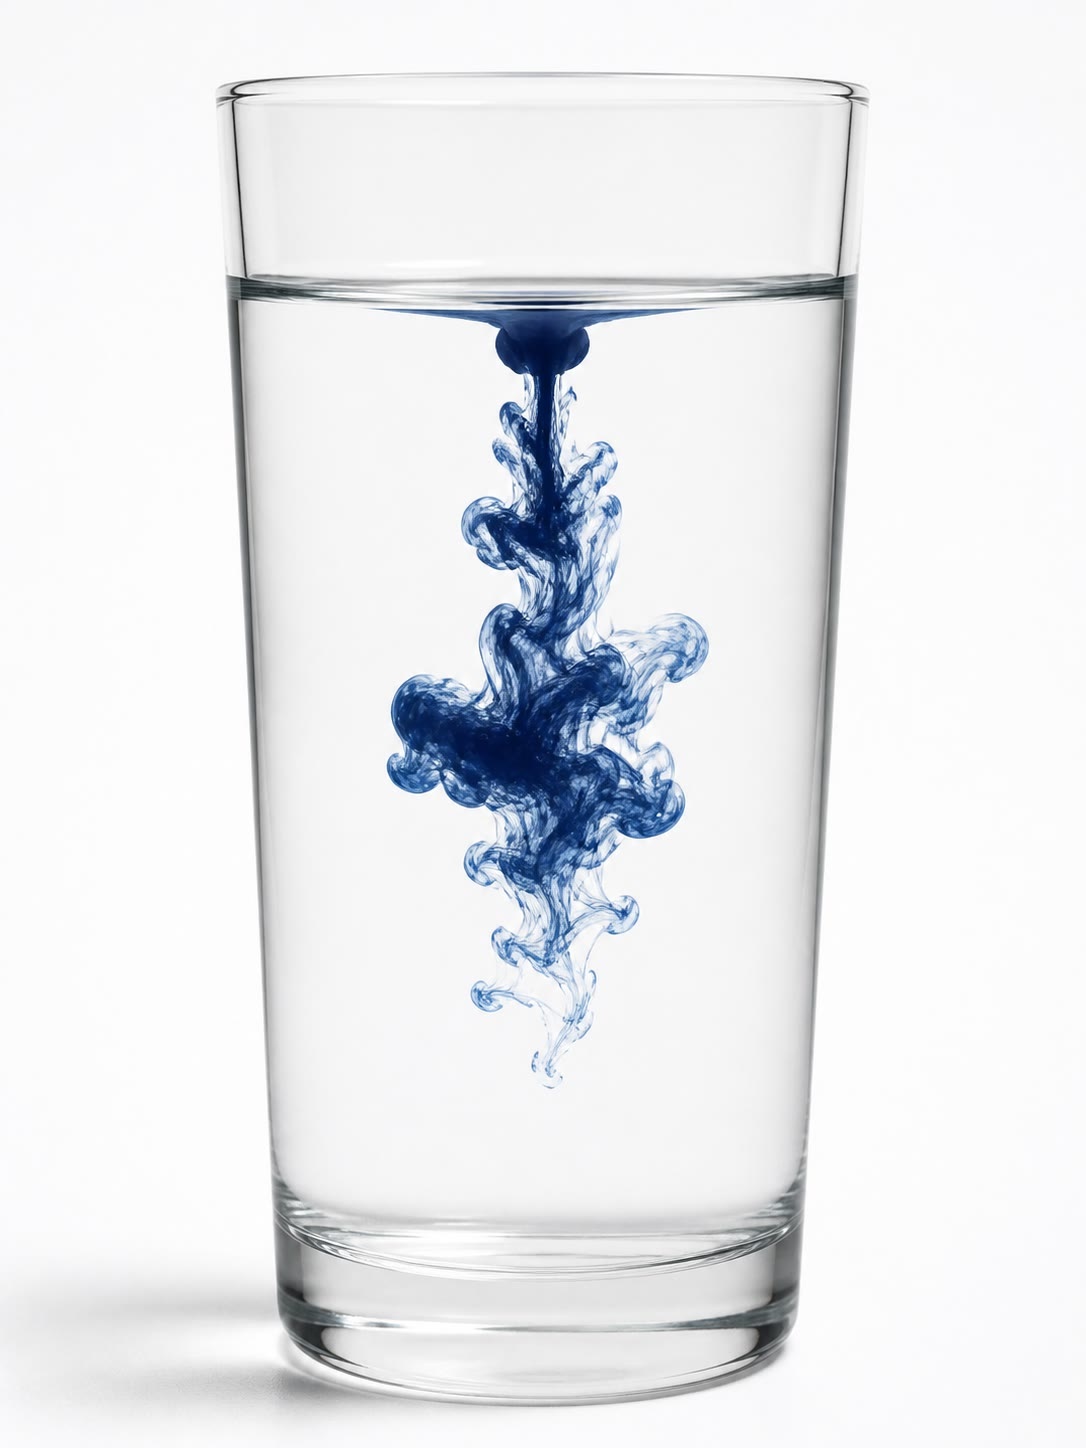
\includegraphics[width=0.58\linewidth]{images/book4/ai/b4-24-ink-drop-water.jpg}

{\small Inkt losgelaten in stilstaand water: de scherpe wolk vervaagt en
spreidt zich
uit naarmate haar moleculen diffunderen --- over millimeters in een minuut,
centimeters
in een uur.}
\end{omfigure}

\section{Deeltjesdichtheid, stroomdichtheid en de wet van Fick}

\begin{definition}[Dichtheid en deeltjesstroom]\label{def:b2:particle-diffusion:flux}
Voor een soort deeltjes (moleculen, ionen, atomen in een vaste stof) is de
\emph{aantalsdichtheid}\index{aantalsdichtheid} $n(M,t)$ het aantal
deeltjes per volume-eenheid rond $M$ (in \unit{m^{-3}}; de molaire
concentratie is $c = n/N_A$). De \emph{deeltjesstroomdichtheid}\index{deeltjes
stroomdichtheid} $\vect{j}_N$ is de vector
zodanig dat het aantal deeltjes dat een georiënteerd oppervlakte-element
$\dd\vect S$ oversteekt in $\dd t$ gelijk is aan
$\vect{j}_N\cdot\dd\vect S\,\dd t$ (in
\unit{m^{-2}.s^{-1}}): de \emph{deeltjesflux} door een oppervlak $S$ is
$\Phi_N = \iint_S \vect{j}_N\cdot\dd\vect S$, het aantal deeltjes per
seconde door $S$. Voor deeltjes die door een fluïdum met snelheid $\vect v$
worden meegevoerd, is
$\vect{j}_N = n\vect v$ (convectie); diffusie is het transport dat
in een fluïdum in rust overblijft.
\end{definition}

\begin{theorem}[Wet van Fick]\label{thm:b2:particle-diffusion:fick}
In een midden in rust, waar de dichtheid niet gelijkmatig is, verschijnt een
deeltjesstroom, evenredig met en tegengesteld aan de \omterm{def:b2:maxwell-equations:operators}{gradiënt} van de
dichtheid:
\[
\vect{j}_N = -D\,\vect{\operatorname{grad}}\,n ,
\]
waarin de \emph{diffusiecoëfficiënt}\index{diffusiecoëfficiënt}
$D > 0$ (in \unit{m^2/s}) van de diffunderende soort, van het
midden en van de temperatuur afhangt. Deeltjes gaan de
dichtheidsgradiënt \emph{af}, van de dichtere naar de ijlere gebieden, met
een tempo dat door $D$ wordt bepaald.
\end{theorem}

\begin{proof}
Fenomenologisch (een ervaringswet, zoals die van Ohm): lineair in de
\omterm{def:b2:maxwell-equations:operators}{gradiënt} voor kleine \omterm{def:b2:maxwell-equations:operators}{gradiënten}, isotroop in een isotroop midden, en
met het teken dat de ervaring oplegt. Het toevalswandelingsmodel van
\cref{sec:b2:particle-diffusion:microscopic} leidt haar af, en $D$ erbij,
uit de moleculaire beweging.
\end{proof}

\begin{example}[Ordes van grootte van $D$]\label{ex:b2:particle-diffusion:orders}
Gassen: $D \sim \qty{1e-5}{m^2/s}$ (waterdamp in lucht
\qty{2.5e-5}{m^2/s}, een parfummolecuul \qty{5e-6}{m^2/s}). Vloeistoffen:
$D \sim \qty{1e-9}{m^2/s}$ (zuurstof in water \qty{2e-9}{m^2/s}, suiker
\qty{5e-10}{m^2/s}, een eiwit \qty{1e-10}{m^2/s}). Vaste stoffen: minuscuul en
steil stijgend met de temperatuur, $D = D_0\,\eu^{-E_{\text{a}}/k_BT}$
(boor in silicium: \qty{1.5e-17}{m^2/s} bij \qty{1100}{\celsius},
onmeetbaar klein bij kamertemperatuur --- en daarom houdt een transistor,
eenmaal gemaakt, zijn doteringsprofiel decennialang). Vier ordes van
grootte van gas naar vloeistof, acht of meer van vloeistof naar vaste stof.
\end{example}

\section{De deeltjesbalans en de diffusievergelijking}

\begin{theorem}[Plaatselijke deeltjesbalans]\label{thm:b2:particle-diffusion:balance}
Als de deeltjes noch worden gemaakt noch vernietigd, geldt
\[
\frac{\partial n}{\partial t} + \operatorname{div}\vect{j}_N = 0 ;
\]
met een bron die $\sigma$ deeltjes per volume-eenheid en per tijdseenheid maakt
(een scheikundige reactie, een absorptie),
$\partial_t n +
\operatorname{div}\vect{j}_N = \sigma$. In één dimensie
(dichtheid en
stroom die alleen van $x$ afhangen): $\partial_t n + \partial_x j_N = 0$.
\end{theorem}

\begin{proof}
Neem de plak tussen $x$ en $x + \dd x$, met doorsnede $S$: zij bevat
$n\,S\,\dd x$ deeltjes; in $\dd t$ komen er $j_N(x)S\,\dd t$ binnen door het
linkervlak en vertrekken er $j_N(x + \dd x)S\,\dd t$ door het rechter, zodat
$\partial_t n\,S\,\dd x\,\dd t = -(j_N(x+\dd x) - j_N(x))S\,\dd t =
-\partial_x j_N\,\dd x\,S\,\dd t$.
In drie dimensies geeft dezelfde telling op
een doosje de \omterm{def:b2:maxwell-equations:operators}{divergentie} (de flux uit een gesloten oppervlak per
volume-eenheid, \cref{ch:b2:maxwell-equations}), of rechtstreeks: voor elk vast
volume $V$ geldt
$\dd/\dd t \iiint_V n\,\dd\tau = -\iint_{\partial V}
\vect{j}_N\cdot\dd\vect S = -\iiint_V \operatorname{div}\vect{j}_N\,\dd\tau$
volgens de \omterm{thm:b2:maxwell-equations:theorems}{stelling van Ostrogradski}.
\end{proof}

\begin{omfigure}
\begin{tikzpicture}[scale=1.0, >=stealth]
  \draw[thick] (0,0) rectangle (5,2);
  \fill[omDef!12] (2.2,0) rectangle (2.9,2);
  \draw[omDef, thick] (2.2,0) -- (2.2,2);
  \draw[omDef, thick] (2.9,0) -- (2.9,2);
  \node[font=\scriptsize, below left] at (2.25,0) {$x$};
  \node[font=\scriptsize, below right] at (2.85,0) {$x + \dd x$};
  \draw[->, omExo, very thick] (1.0,1) -- (2.1,1) node[midway, above, font=\scriptsize] {$j_N(x)$};
  \draw[->, omExo, very thick] (3.0,1) -- (4.1,1) node[midway, above, font=\scriptsize] {$j_N(x + \dd x)$};
  \node[font=\scriptsize] at (2.55,1.6) {$n$};
  \node[font=\scriptsize, right] at (5.1,1) {doorsnede $S$};
  \draw[->] (0,-0.7) -- (5.5,-0.7) node[right, font=\scriptsize] {$x$};
\end{tikzpicture}

{\small De eendimensionale balans: de plak tussen $x$ en $x + \dd
x$ wint
wat er links binnenkomt en verliest wat er rechts vertrekt;
het verschil is de verandering van $n$ binnenin.}
\end{omfigure}

\begin{theorem}[Diffusievergelijking]\label{thm:b2:particle-diffusion:equation}
De wet van Fick en de balans samen geven, voor gelijkmatige $D$,
\[
\frac{\partial n}{\partial t} = D\,\Delta n + \sigma ,
\qquad\text{in één dimensie}\quad
\frac{\partial n}{\partial t} = D\,\frac{\partial^2 n}{\partial x^2} + \sigma .
\]
Deze \emph{diffusievergelijking}\index{diffusievergelijking} is lineair
(oplossingen tellen op), van eerste orde in de tijd en van tweede orde in de ruimte
--- geen \omterm{thm:b2:waves-on-strings:equation}{golfvergelijking}: zij heeft geen voortplantingssnelheid, maar een
kenmerkende betrekking tussen lengte en tijd,
\[
L \sim \sqrt{D t}, \qquad t \sim \frac{L^2}{D} :
\]
over twee keer de afstand diffunderen duurt vier keer zo lang.
\end{theorem}

\begin{proof}
$\partial_t n = -\operatorname{div}(-D\,\vect{\operatorname{grad}}\,n) +
\sigma = D\operatorname{div}\vect{\operatorname{grad}}\,n + \sigma = D\Delta
n + \sigma$.
Vergelijk voor de schalen $n/t$ met $Dn/L^2$.
\end{proof}

\begin{remark}[Diffusie is onomkeerbaar]\label{rem:b2:particle-diffusion:irreversible}
Verander $t$ in $-t$ in de \omterm{thm:b2:waves-on-strings:equation}{golfvergelijking},
$\partial_t^2 u = c^2
\partial_x^2 u$, en zij blijft dezelfde: een film van
een golf die achterstevoren loopt is
een mogelijke golf. Doe hetzelfde in de \omterm{thm:b2:particle-diffusion:equation}{diffusievergelijking} en het teken van
het linkerlid keert om: $n(x,-t)$ is \emph{geen} oplossing. Een wolk die
zich uitspreidt is natuurlijk; een wolk die zich spontaan tot een kristal verzamelt
is dat niet --- diffusie heeft een tijdpijl, de pijl van de tweede hoofdwet
(\cref{ch:b2:heat-conduction} berekent de entropie die zij maakt). De
vergelijking toont ook dat diffusie glad strijkt: waar $n$ plaatselijk een
maximum is ($\partial_x^2 n < 0$) daalt zij, waar zij een minimum is
stijgt zij.
\end{remark}

\begin{example}[Hoe lang duurt het?]\label{ex:b2:particle-diffusion:times}
$t \sim L^2/D$. Zuurstof door een cel, $L = \qty{10}{\micro m}$ in water:
$10^{-10}/2 \times 10^{-9} = \qty{0.05}{s}$ --- diffusie voedt een cel met
gemak; door \qty{1}{mm} weefsel: \qty{500}{s} --- te traag, en daarom
is niets levends dikker dan een fractie van een millimeter zonder
bloedvaten. Suiker door een kop ongeroerde thee, $L = \qty{5}{cm}$:
$2.5 \times 10^{-3}/5 \times 10^{-10} = 5 \times 10^6\,\unit{s}$, twee maanden
--- roer. Een parfum door een kamer, alleen door diffusie, \qty{5}{m} in
lucht: $25/10^{-5} = \qty{3e6}{s}$, een maand; u ruikt het binnen een minuut
omdat de lucht beweegt: \emph{convectie} draagt, diffusie doet alleen
de laatste millimeters.
\end{example}

\section{Kenmerkende oplossingen}

\begin{proposition}[Stationair regime: het membraan]\label{prop:b2:particle-diffusion:membrane}
Tussen twee reservoirs die op $n_1$ en $n_2$ worden gehouden, door een membraan met
dikte $e$ en oppervlak $S$, is de stationaire dichtheid lineair,
\[
n(x) = n_1 + (n_2 - n_1)\frac{x}{e}, \qquad
j_N = D\,\frac{n_1 - n_2}{e}, \qquad
\Phi_N = \frac{n_1 - n_2}{R_{\text{d}}}, \quad R_{\text{d}} = \frac{e}{DS}:
\]
het membraan heeft een \emph{diffusieve weerstand} $e/DS$, net zoals een draad
$\ell/\gamma S$ heeft --- weerstanden in serie tellen op, en een dun membraan
met kleine $D$ kan toch overheersen.
\end{proposition}

\begin{proof}
Stationair, eendimensionaal, zonder bron: $\partial_x^2 n = 0$, zodat $n$
affien is; $j_N = -D\,\dd n/\dd x$ is gelijkmatig.
\end{proof}

\begin{proposition}[Stationair regime: bolvormige meetkunde]\label{prop:b2:particle-diffusion:sphere}
Rond een bol met straal $a$ waarvan het oppervlak op $n_0$ wordt gehouden, in een
midden waar $n \to 0$ ver weg, is de stationaire dichtheid
\[
n(r) = n_0\,\frac{a}{r}, \qquad
\Phi_N = 4\pi D a\,n_0 :
\]
groeit de totale vrijgekomen (of opgenomen, met omgekeerde tekens) stroom
met de \emph{straal} van de bol, niet met haar oppervlak --- de
meetkunde van een diffusieve put is die van een elektrostatische capaciteit.
\end{proposition}

\begin{proof}
$\Delta n = \frac{1}{r^2}\frac{\dd}{\dd r}(r^2\,\dd n/\dd r) = 0$ geeft
$n = A + B/r$; de randvoorwaarden leggen $A = 0$, $B = n_0 a$ vast; dan is
$\Phi_N = -4\pi r^2 D\,\dd n/\dd r = 4\pi D n_0 a$ bij elke $r$ (geen
opeenhoping in het stationaire regime).
\end{proof}

\begin{omfigure}
\begin{tikzpicture}
  \begin{axis}[omaxis, width=5.6cm, height=4.2cm, xmin=-0.3, xmax=1.4, ymin=0, ymax=1.3,
    xlabel={$x/e$}, ylabel={$n/n_1$}, xtick={0,1}, ytick={1}, clip=false]
    \addplot[omDef, thick, domain=0:1] {1-0.7*x};
    \draw[dashed] (axis cs:1,0) -- (axis cs:1,0.3);
    \node[font=\scriptsize, anchor=west] at (axis cs:1.03,0.3) {$n_2$};
    \node[font=\scriptsize, omExo, anchor=west] at (axis cs:0.3,1.0) {$j_N = D(n_1 - n_2)/e$};
    \draw[->, omExo, thick] (axis cs:0.3,0.45) -- (axis cs:0.7,0.45);
  \end{axis}
  \begin{axis}[omaxis, width=5.6cm, height=4.2cm, xmin=0, xmax=5, ymin=0, ymax=1.3, xshift=5.9cm,
    xlabel={$r/a$}, ylabel={$n/n_0$}, xtick={1,2,3,4}, ytick={1}, clip=false]
    \addplot[omDef, thick, domain=1:5, samples=60] {1/x};
    \draw[dashed] (axis cs:1,0) -- (axis cs:1,1);
    \node[font=\scriptsize, omExo] at (axis cs:3,0.6) {$n = n_0 a/r$};
  \end{axis}
\end{tikzpicture}

{\small Stationaire profielen. Links: door een membraan is de dichtheid
lineair en de stroom gelijkmatig. Rechts: rond een bol daalt de dichtheid
als $1/r$; de totale stroom $4\pi D a n_0$ is evenredig met de
straal.}
\end{omfigure}

\begin{proposition}[De uitdijende gaussische verdeling]\label{prop:b2:particle-diffusion:gaussian}
$N$ deeltjes per oppervlakte-eenheid die op $t = 0$ in het vlak $x = 0$ van
een oneindig midden worden losgelaten, spreiden zich als
\[
n(x,t) = \frac{N}{\sqrt{4\pi D t}}\,\exp\Big(-\frac{x^2}{4Dt}\Big) :
\]
een gaussische verdeling met standaardafwijking $\sigma(t) = \sqrt{2Dt}$,
met constante
oppervlakte $N$ (de deeltjes blijven behouden) en dalende piek
$\propto
1/\sqrt t$. In drie dimensies spreiden $N$ deeltjes die in een punt
worden losgelaten
zich als $n = N\,(4\pi Dt)^{-3/2}\exp(-r^2/4Dt)$, met
$\langle r^2
\rangle = 6Dt$. Een puls deeltjes losgelaten aan het
\emph{oppervlak} van
een halfruimte (die zij niet kunnen verlaten) geeft twee keer de
bovenstaande uitdrukking
voor $x > 0$.
\end{proposition}

\begin{proof}
Vul in: met $u = x^2/4Dt$ is $\partial_t n = n\,(-1/2t + u/t)$ en
$D\,\partial_x^2 n = D\,n\,(-1/2Dt + x^2/4D^2t^2) = n\,(-1/2t + u/t)$;
gelijk. De normering $\int n\,\dd x = N$ volgt uit
$\int
\eu^{-x^2/4Dt}\dd x = \sqrt{4\pi Dt}$, en $\int x^2 n\,\dd x/N = 2Dt$.
De eenduidigheid (gegeven de beginpuls) wordt aangenomen.
\end{proof}

\begin{omfigure}
\begin{tikzpicture}
  \begin{axis}[omaxis, width=9cm, height=4.8cm, xmin=-4.2, xmax=4.2, ymin=0, ymax=1.05,
    xlabel={$x/\sqrt{2Dt_1}$}, ylabel={$n$}, ytick=\empty, xtick={-4,-2,2,4}, clip=false,
    legend style={font=\scriptsize, at={(0.97,0.95)}, anchor=north east, draw=none, fill=none}]
    \addplot[omDef, thick, domain=-4.2:4.2, samples=100] {exp(-x*x/2)};
    \addlegendentry{$t_1$}
    \addplot[omThm, thick, domain=-4.2:4.2, samples=100] {0.5*exp(-x*x/8)};
    \addlegendentry{$4t_1$}
    \addplot[omExo, thick, domain=-4.2:4.2, samples=100] {0.25*exp(-x*x/32)};
    \addlegendentry{$16t_1$}
  \end{axis}
\end{tikzpicture}

{\small De gaussische oplossing op drie tijdstippen: de breedte groeit als
$\sqrt t$, de piek daalt als $1/\sqrt t$, de oppervlakte (het aantal
deeltjes) blijft dezelfde.}
\end{omfigure}

\begin{proposition}[Vaste oppervlakteconcentratie]\label{prop:b2:particle-diffusion:erfc}
Een halfruimte $x > 0$ die aanvankelijk leeg is en waarvan het oppervlak op
de dichtheid $n_0$ wordt gehouden vanaf $t = 0$ (een gas in aanraking met
een vaste stof die
het oplost), vult zich als
\[
n(x,t) = n_0\,\operatorname{erfc}\Big(\frac{x}{2\sqrt{Dt}}\Big),
\qquad
\operatorname{erfc}(u) = \frac{2}{\sqrt\pi}\int_u^{\infty}\eu^{-s^2}\dd s,
\]
de \emph{complementaire foutfunctie}, die van $1$ bij $u =
0$ daalt tot
$0.16$ bij $u = 1$ en $0.005$ bij $u = 2$: de \omterm{def:b2:dispersion-wave-packets:complex}{indringdiepte} is
opnieuw $\sim 2\sqrt{Dt}$, en het totale aantal opgenomen deeltjes per
oppervlakte-eenheid is $2n_0\sqrt{Dt/\pi}$.
\end{proposition}

\begin{proof}
Zoek $n = f(u)$ met $u = x/2\sqrt{Dt}$: de vergelijking wordt
$f'' + 2uf' = 0$, dus $f' \propto \eu^{-u^2}$ en $f$ is een foutfunctie;
de voorwaarden $f(0) = n_0$, $f(\infty) = 0$ kiezen
$\operatorname{erfc}$. Het opgenomen aantal is
$\int_0^\infty n\,\dd x =
n_0\,2\sqrt{Dt}\int_0^\infty\operatorname{erfc}(u)\dd u = 2n_0\sqrt{Dt/\pi}$.
\end{proof}

\begin{example}[Staal harden]\label{ex:b2:particle-diffusion:carburising}
Een stalen onderdeel dat bij \qty{900}{\celsius} in een koolstofrijk gas
wordt gehouden, neemt
aan zijn oppervlak koolstof op; met $D = \qty{5e-12}{m^2/s}$ voor koolstof in heet
ijzer geven vier uur $2\sqrt{Dt} = \qty{0.5}{mm}$: een harde huid van een halve
millimeter op een taaie kern --- het \emph{inzetharden} van tandwielen en
lagers, op de erfc-profiel getimed.
\end{example}

\section{Het microscopische beeld: de
toevalswandeling}\label{sec:b2:particle-diffusion:microscopic}

\begin{proposition}[Toevalswandeling en de diffusiecoëfficiënt]\label{prop:b2:particle-diffusion:walk}
Een deeltje dat een stap van lengte $\ell$ in een willekeurige richting zet
om de $\tau$ (een molecuul tussen twee botsingen), heeft na $N =
t/\tau$
stappen een
gemiddelde kwadratische verplaatsing
\[
\langle x^2\rangle = N\ell^2 = \frac{\ell^2}{\tau}\,t
\quad\text{(één dimensie)}, \qquad
\langle r^2\rangle = 3\langle x^2\rangle \quad\text{(drie dimensies)}.
\]
Vergelijking met de gaussische oplossing, $\langle x^2\rangle = 2Dt$, geeft:
\[
D = \frac{\ell^2}{2\tau} \quad\text{(1D)}, \qquad
D = \frac{\ell^2}{6\tau} = \frac{\ell\,v^*}{6}\ \sim\ \frac{\ell\,v^*}{3}
\quad\text{(3D, met } v^* = \ell/\tau\text{; kinetische theorie: } \tfrac13) .
\]
De afstand van de wandelaar groeit als $\sqrt t$, niet als $t$: om twee keer
zo ver te gaan
heeft hij vier keer zoveel stappen nodig.
\end{proposition}

\begin{proof}
$x = \sum_i \epsilon_i\ell$ met onafhankelijke $\epsilon_i = \pm1$ (1D):
$\langle x^2\rangle = \sum_{i,j}\langle\epsilon_i\epsilon_j\rangle\ell^2 =
N\ell^2$,
waarbij de kruistermen tot nul middelen. De verdeling van $x$
nadert voor grote $N$ een gaussische (de centrale limietstelling, waarvan het
bewijs bij de kansrekening hoort) --- en daarom is de
macroscopische wet de \omterm{thm:b2:particle-diffusion:equation}{diffusievergelijking}; de wet van Fick zelf volgt
uit het tellen van de wandelaars die een vlak van beide zijden oversteken:
$j_N \approx
-\tfrac12\ell v^*\,\partial_x n$ (een zorgvuldiger middeling
geeft $1/3$ in
drie dimensies).
\end{proof}

\begin{omfigure}
\begin{tikzpicture}[scale=0.85]
  \draw[omDef, thin] plot coordinates {(0,0) (-0.1,-0.15) (-0.16,0.02) (-0.24,-0.14) (-0.1,-0.03) (-0.28,-0.05) (-0.46,-0.04) (-0.61,-0.14) (-0.73,-0.01) (-0.74,0.17) (-0.86,0.3) (-0.78,0.14) (-0.7,0.3) (-0.75,0.47) (-0.86,0.33) (-0.82,0.15) (-0.64,0.14) (-0.58,-0.03) (-0.76,0.01) (-0.93,-0.04) (-1.06,-0.16) (-1.06,0.02) (-1.11,-0.16) (-1.15,-0.33) (-0.97,-0.36) (-1.05,-0.2) (-1.22,-0.14) (-1.27,-0.31) (-1.28,-0.49) (-1.2,-0.33) (-1.02,-0.31) (-0.98,-0.49) (-0.81,-0.44) (-0.96,-0.55) (-0.95,-0.37) (-1.12,-0.43) (-1.3,-0.45) (-1.44,-0.34) (-1.37,-0.18) (-1.48,-0.32) (-1.52,-0.49) (-1.58,-0.32) (-1.4,-0.36) (-1.31,-0.51) (-1.45,-0.4) (-1.5,-0.57) (-1.37,-0.44) (-1.51,-0.56) (-1.68,-0.61) (-1.74,-0.78) (-1.59,-0.88) (-1.73,-0.77) (-1.64,-0.93) (-1.78,-1.05) (-1.6,-1.03) (-1.72,-0.91) (-1.59,-0.79) (-1.75,-0.86) (-1.88,-0.73) (-1.77,-0.58) (-1.71,-0.75) (-1.55,-0.67) (-1.39,-0.58) (-1.34,-0.41) (-1.19,-0.52) (-1.36,-0.57) (-1.54,-0.56) (-1.67,-0.43) (-1.53,-0.33) (-1.7,-0.28) (-1.76,-0.11) (-1.89,0.02) (-1.76,0.14) (-1.59,0.08) (-1.55,-0.09) (-1.71,-0.02) (-1.88,-0.09) (-1.7,-0.07) (-1.52,-0.11) (-1.43,0.04) (-1.53,0.19) (-1.53,0.01) (-1.57,-0.17) (-1.48,-0.33) (-1.4,-0.16) (-1.46,-0.33) (-1.29,-0.28) (-1.11,-0.29) (-0.93,-0.25) (-0.84,-0.1) (-0.66,-0.11) (-0.74,-0.27) (-0.56,-0.22) (-0.55,-0.04) (-0.67,-0.18) (-0.57,-0.03) (-0.42,-0.13) (-0.59,-0.06) (-0.47,-0.2) (-0.65,-0.2) (-0.56,-0.04) (-0.52,-0.22) (-0.34,-0.21) (-0.29,-0.39) (-0.34,-0.21) (-0.21,-0.08) (-0.18,0.09) (-0.35,0.15) (-0.34,0.33) (-0.35,0.15) (-0.39,-0.03) (-0.43,0.15) (-0.38,0.33) (-0.47,0.17) (-0.61,0.06) (-0.48,-0.06) (-0.44,0.11) (-0.32,0.25) (-0.49,0.18) (-0.31,0.17) (-0.47,0.24) (-0.6,0.37) (-0.44,0.44) (-0.48,0.61) (-0.5,0.43) (-0.47,0.61) (-0.58,0.75) (-0.74,0.84) (-0.87,0.96) (-0.83,0.79) (-0.67,0.69) (-0.8,0.56) (-0.98,0.59) (-1.14,0.51) (-1.27,0.38) (-1.27,0.2) (-1.12,0.1) (-1.27,0.2) (-1.38,0.35) (-1.21,0.4) (-1.37,0.47) (-1.54,0.52) (-1.46,0.68) (-1.56,0.53) (-1.4,0.45) (-1.36,0.27) (-1.19,0.22) (-1.03,0.13) (-0.86,0.06) (-0.96,-0.1) (-1.14,-0.09) (-1.26,-0.22) (-1.08,-0.26) (-0.92,-0.2) (-0.74,-0.16) (-0.81,0) (-0.95,-0.11) (-1.06,-0.26) (-0.92,-0.14) (-1.07,-0.24) (-1.23,-0.33) (-1.27,-0.51) (-1.12,-0.61) (-1.04,-0.77) (-1.07,-0.6) (-0.93,-0.49) (-0.94,-0.67) (-0.78,-0.75) (-0.93,-0.85) (-0.78,-0.94) (-0.6,-0.93) (-0.6,-1.11) (-0.73,-1.24) (-0.63,-1.39) (-0.72,-1.24) (-0.66,-1.41) (-0.66,-1.23) (-0.48,-1.21) (-0.34,-1.33) (-0.41,-1.49) (-0.35,-1.65) (-0.21,-1.54) (-0.04,-1.48) (0.14,-1.44) (0.11,-1.27) (-0.01,-1.4) (0.15,-1.31) (-0.03,-1.26) (0.13,-1.36) (0.12,-1.18) (0.29,-1.13) (0.42,-1) (0.44,-1.18) (0.6,-1.26) (0.68,-1.42) (0.51,-1.39) (0.47,-1.21) (0.49,-1.39) (0.59,-1.25) (0.69,-1.39) (0.87,-1.43) (0.75,-1.3) (0.73,-1.48) (0.59,-1.37) (0.61,-1.55) (0.54,-1.71) (0.37,-1.63) (0.52,-1.53) (0.67,-1.63) (0.78,-1.78) (0.75,-1.6) (0.79,-1.42) (0.83,-1.6) (0.68,-1.5) (0.56,-1.63) (0.68,-1.49) (0.84,-1.56) (0.97,-1.43) (1.11,-1.31) (1.08,-1.49) (1.02,-1.33) (1.13,-1.47) (0.95,-1.44) (0.9,-1.27) (1.01,-1.13) (0.98,-1.3) (0.86,-1.18) (0.78,-1.01) (0.69,-1.17) (0.87,-1.15) (0.98,-1.28) (1.13,-1.38) (1,-1.51) (1.13,-1.38) (1.17,-1.55) (1.23,-1.38) (1.19,-1.21) (1.29,-1.36) (1.43,-1.47) (1.42,-1.65) (1.28,-1.76) (1.13,-1.65) (1.03,-1.8) (1.2,-1.85) (1.16,-1.68) (0.99,-1.76) (1.1,-1.9) (1.11,-2.08) (0.93,-2.11) (1.01,-1.95) (0.99,-2.13) (0.81,-2.14) (0.98,-2.18) (0.85,-2.05) (1.03,-2.1) (1.04,-1.92) (1.18,-2.03) (1.36,-2.01) (1.54,-2.04) (1.37,-1.98) (1.53,-1.92) (1.37,-1.84) (1.51,-1.72) (1.45,-1.55) (1.6,-1.46) (1.75,-1.36) (1.86,-1.22) (1.81,-1.39) (1.98,-1.34) (1.94,-1.16) (1.8,-1.05) (1.85,-1.22) (2.03,-1.22) (1.91,-1.08) (1.83,-0.92) (1.72,-1.05) (1.79,-0.89) (1.74,-1.06) (1.57,-1.12) (1.39,-1.15) (1.23,-1.22) (1.41,-1.22) (1.36,-1.05) (1.18,-1.06) (1,-1.06) (1.09,-1.22) (1.08,-1.04) (1.25,-1.1) (1.33,-0.95) (1.3,-0.77) (1.31,-0.95) (1.28,-0.77) (1.14,-0.88) (1.04,-1.03) (0.95,-0.88) (1.08,-0.75) (1.22,-0.86) (1.26,-1.03) (1.08,-1.01) (1.12,-1.19) (0.95,-1.11) (1.12,-1.03) (1.17,-1.2) (1.27,-1.05) (1.26,-1.23) (1.44,-1.21) (1.42,-1.03) (1.3,-0.9) (1.38,-1.06) (1.56,-1.02) (1.6,-1.2) (1.76,-1.28) (1.6,-1.36) (1.46,-1.26) (1.55,-1.41) (1.61,-1.58) (1.79,-1.58) (1.73,-1.41) (1.61,-1.27) (1.65,-1.1) (1.8,-1.01) (1.66,-1.12) (1.52,-1.23) (1.36,-1.31) (1.48,-1.45) (1.3,-1.41) (1.34,-1.24) (1.33,-1.06) (1.16,-1.09) (1.1,-0.92) (1.12,-0.74) (1.04,-0.91) (1.04,-0.73) (0.93,-0.58) (0.97,-0.41) (0.81,-0.49) (0.65,-0.41) (0.65,-0.23) (0.7,-0.05) (0.55,-0.15) (0.73,-0.11) (0.82,-0.27) (0.92,-0.42) (0.87,-0.25) (1.05,-0.23) (1.08,-0.41) (1.19,-0.27) (1.22,-0.45) (1.39,-0.42) (1.57,-0.41) (1.39,-0.38) (1.38,-0.56) (1.36,-0.74) (1.27,-0.9) (1.44,-0.82) (1.26,-0.79) (1.4,-0.91) (1.33,-1.07) (1.2,-1.2) (1.03,-1.16) (0.86,-1.09) (0.75,-0.95) (0.57,-0.98) (0.75,-1.02) (0.81,-1.18) (0.69,-1.05) (0.86,-1.11) (0.74,-1.24) (0.6,-1.35) (0.43,-1.39) (0.27,-1.49) (0.43,-1.39) (0.58,-1.3) (0.4,-1.33) (0.46,-1.15) (0.51,-1.33) (0.44,-1.16) (0.54,-1.02) (0.49,-1.19) (0.58,-1.03) (0.44,-1.15) (0.46,-0.97) (0.64,-0.94) (0.82,-0.94) (0.91,-0.79) (0.92,-0.97) (0.75,-0.93) (0.59,-0.84) (0.62,-0.66) (0.6,-0.48) (0.53,-0.65) (0.45,-0.49) (0.62,-0.43) (0.62,-0.25) (0.66,-0.07) (0.5,-0.15) (0.62,-0.28) (0.44,-0.24) (0.27,-0.3) (0.28,-0.48) (0.39,-0.62)};
  \fill[omExo] (0,0) circle (2.5pt);
  \fill[omThm] (0.39,-0.62) circle (2.5pt);
  \draw[thin, gray] (0,0) -- (-2.4,1.2);
  \node[font=\scriptsize, omExo, anchor=east] at (-2.4,1.2) {begin};
  \draw[thin, gray] (0.39,-0.62) -- (2.5,-1.3);
  \node[font=\scriptsize, omThm, anchor=west] at (2.5,-1.3) {na $400$ stappen};
  \draw[<->, thin] (-2.3,-2.5) -- (2.3,-2.5) node[midway, below, font=\scriptsize] {$\sim \ell\sqrt N$};
\end{tikzpicture}

{\small Een toevalswandeling van $400$ stappen met lengte $\ell$: de wandelaar is
maar zo'n $20\ell$ van zijn begin gedwaald --- de $\sqrt N$-wet die
diffusie zo traag over lange afstanden en zo snel over korte maakt.}
\end{omfigure}

\begin{example}[Van moleculen naar $D$]\label{ex:b2:particle-diffusion:kinetic}
Lucht bij kamertemperatuur: gemiddelde vrije weglengte $\ell \approx \qty{70}{nm}$,
gemiddelde snelheid $v^* \approx \qty{500}{m/s}$:
$D \approx \ell v^*/3 =
\qty{1.2e-5}{m^2/s}$, zoals gemeten. Om \qty{1}{m}
te diffunderen heeft een molecuul
$N = (L/\ell)^2 = 2 \times 10^{14}$ botsingen nodig, dus
$N\ell/v^*
\approx \qty{3e4}{s}$ --- acht uur voor een reis die het in
\qty{2}{ms} zou maken als het rechtdoor vloog. In een vloeistof gehoorzaamt
een bol met straal $a$
die door de moleculen wordt gebeukt aan de betrekking van Stokes--Einstein
$D =
k_BT/6\pi\eta a$ (Einstein 1905): voor suiker is
$a \approx \qty{0.4}{nm}$
in water, $D = \qty{5e-10}{m^2/s}$; voor een korrel van \qty{1}{\micro m},
$\qty{4e-13}{m^2/s}$, een verplaatsing van een micrometer per seconde ---
de brownse beweging die Perrin mat om het getal van Avogadro te tellen. In
een vaste stof springt een atoom pas naar een naburige plaats wanneer een thermische
fluctuatie de activeringsenergie levert: $D = D_0\,\eu^{-E_{\text{a}}/k_BT}$,
verdubbelend om de enkele tientallen kelvin nabij \qty{1000}{\celsius}.
\end{example}

\begin{method}[Diffusieschattingen]\label{meth:b2:particle-diffusion:method}
(1) Bepaal $D$ (gas $10^{-5}$, vloeistof $10^{-9}$, vaste stof arrhenius).
(2) Tijd of afstand: $t \sim L^2/D$, $L \sim \sqrt{Dt}$ (met exact
$\sqrt{2Dt}$ voor de gaussische breedte, $2\sqrt{Dt}$ voor de erfc-diepte).
(3) Stationair: lineair in een plak ($R_{\text{d}} = e/DS$), $1/r$ rond een
bol ($\Phi = 4\pi D a\,\Delta n$), $\ln r$ rond een cilinder. (4)
Overgangsverschijnsel: gaussisch voor een puls, erfc voor een vastgehouden
oppervlak; tel op.
(5) Vraag u af of convectie niet overheerst. (6) Microscopische controle:
$D \sim \ell v^*/3$.
\end{method}

\section{Opgaven}

\begin{exercise}[$\star$]\label{exo:b2:particle-diffusion:1}
Diffusietijden $L^2/D$: een suikerklontje op de bodem van een kop van \qty{5}{cm}
($D = \qty{5e-10}{m^2/s}$); parfum door een kamer van \qty{5}{m}
($D =
\qty{5e-6}{m^2/s}$); zuurstof door \qty{1}{mm} weefsel en door een
cel van \qty{10}{\micro m} ($D = \qty{2e-9}{m^2/s}$). Welke van deze doet
diffusie werkelijk?
\end{exercise}

\begin{exercise}[$\star$]\label{exo:b2:particle-diffusion:2}
Een membraan van \qty{1}{\micro m} dik en \qty{1}{cm^2} groot, met
$D =
\qty{1e-11}{m^2/s}$ erin, scheidt een oplossing van \qty{1}{mol/m^3}
van zuiver water. \omterm{def:b2:charges-currents-conduction:densities}{Stroomdichtheid}, molaire flux en aantal moleculen
per seconde; diffusieve weerstand; met twee zulke membranen in serie.
\end{exercise}

\begin{exercise}[$\star$]\label{exo:b2:particle-diffusion:3}
Een dunne laag kleurstof ($N = \qty{1e20}{m^{-2}}$) wordt in water losgelaten,
$D = \qty{1e-9}{m^2/s}$. Breedte $\sqrt{2Dt}$ en piekdichtheid na
\qty{1}{s}, \qty{1}{h}, \qty{1}{dag}. Wanneer is de piek gedaald tot
$1\%$ van haar waarde bij \qty{1}{s}?
\end{exercise}

\begin{exercise}[$\star$]\label{exo:b2:particle-diffusion:4}
Luchtmoleculen: $\ell = \qty{70}{nm}$, $v^* = \qty{500}{m/s}$. Schat
$D$; aantal botsingen en tijd om \qty{1}{m} te diffunderen; vergelijk met
de rechtlijnige vlucht. Idem voor een molecuul in water
($\ell \approx
\qty{0.1}{nm}$, $v^* \approx \qty{500}{m/s}$): klopt de
schatting, en
waarom niet precies?
\end{exercise}

\begin{exercise}[$\star\star$]\label{exo:b2:particle-diffusion:5}
\emph{Zuurstof in een weefsel.} Een weefselplaat met dikte $2a$ verbruikt
zuurstof met het gelijkmatige tempo $q$ (per volume-eenheid); haar twee
vlakken worden
op $n_0$ gehouden. (a) Schrijf de stationaire vergelijking met de put en los
haar op. (b) Voorwaarde opdat zuurstof het midden bereikt. (c)
$D = \qty{2e-9}{m^2/s}$,
$n_0 = \qty{0.2}{mol/m^3}$, $q = \qty{0.01}{mol/m^3/s}$: grootste $a$. (d)
Besluit over de onderlinge afstand van haarvaten.
\end{exercise}

\begin{exercise}[$\star\star$]\label{exo:b2:particle-diffusion:6}
\emph{Een oplossende korrel.} Een suikerbol met straal $a = \qty{1}{mm}$
in stilstaand water houdt haar oppervlak op de verzadigingsdichtheid
$n_{\text{s}}
= \qty{5800}{mol/m^3}$; ver weg is het water zuiver;
$D =
\qty{5e-10}{m^2/s}$. (a) Stationair profiel en totale stroom. (b)
Aantal mol in de korrel (dichtheid \qty{1590}{kg/m^3}, molmassa
\qty{342}{g/mol}) en oplostijd (neem de stroom constant).
(c) Waarom is de werkelijke tijd langer, en waarom helpt roeren zo veel?
(d) Toon aan dat het stationaire profiel voor een zeer lange cilinder
logaritmisch is en dat het vraagstuk in een oneindig midden geen oplossing heeft.
\end{exercise}

\begin{exercise}[$\star\star$]\label{exo:b2:particle-diffusion:7}
\emph{Behoud en onomkeerbaarheid.} (a) Toon uit de vergelijking aan
dat $\int n\,\dd x$ constant is en dat $\dd\langle x^2\rangle/\dd t =
2D$
(partieel integreren, $n \to 0$ op oneindig). (b) Toon aan dat
$n(x,-t)$ niet aan de vergelijking voldoet. (c) Wat wordt er van de
gaussische oplossing voor $t < 0$? (d) Toon aan dat $\int n^2\,\dd x$ alleen kan
dalen: diffusie strijkt vlak.
\end{exercise}

\begin{exercise}[$\star\star$]\label{exo:b2:particle-diffusion:8}
\emph{Inzetharden.} Koolstof in heet ijzer, $D = \qty{5e-12}{m^2/s}$ bij
\qty{900}{\celsius}; oppervlak op $n_0$ gehouden. (a) Ga na dat
$n_0
\operatorname{erfc}(x/2\sqrt{Dt})$ de vergelijking oplost. (b) Diepte
waarop
$n = 0.1\,n_0$ na \qty{4}{h} ($\operatorname{erfc}(1.16) = 0.1$).
(c) Tijd voor de dubbele diepte. (d) Bij \qty{950}{\celsius} is $D$ $2.5$
keer groter: uitgespaarde tijd.
\end{exercise}

\begin{exercise}[$\star\star$]\label{exo:b2:particle-diffusion:9}
\emph{Stokes--Einstein.} $D = k_BT/6\pi\eta a$, water
$\eta =
\qty{1e-3}{Pa.s}$, \qty{300}{K}. (a) $D$ voor
$a = \qty{1}{\micro m}$ en
de kwadratisch gemiddelde verplaatsing in \qty{1}{s}, \qty{1}{min}. (b) $D$
voor een eiwit, $a = \qty{3}{nm}$. (c) Suiker heeft $D = \qty{5e-10}{m^2/s}$:
werkzame straal. (d) Hoe geeft het meten van $\langle x^2\rangle$ van een korrel
onder een microscoop het getal van Avogadro?
\end{exercise}

\begin{exercise}[$\star\star\star$]\label{exo:b2:particle-diffusion:10}
\emph{Vertraging van een membraan.} Een membraan met dikte $e$, aanvankelijk
wordt aan één vlak blootgesteld aan $n_1$ op $t = 0$, het andere vlak op
$0$ gehouden. (a) Wat is de uiteindelijke stationaire flux? (b) Beredeneer
dat de flux
op het verre vlak stijgt over een tijd $\sim e^2/D$ (de exacte vertraging is
$e^2/6D$). (c) Een geneesmiddelenpleister met $e = \qty{20}{\micro m}$,
$D =
\qty{1e-13}{m^2/s}$ door de buitenste huidlaag: vertragingstijd. (d)
Waarom
is de vertraging nuttig om $D$ te meten en de stationaire flux om
$D \times$ oplosbaarheid te meten?
\end{exercise}

\begin{exercise}[$\star\star\star$]\label{exo:b2:particle-diffusion:11}
\emph{De volmaakte opnemer.} Een bol met straal $a$ neemt elk
deeltje op dat haar raakt, in een midden dat ver weg op $n_\infty$ staat. (a)
Stationair profiel en totale opgevangen stroom. (b) Een bacterie,
$a =
\qty{1}{\micro m}$, in een suikeroplossing met
$n_\infty = \qty{6e20}{m^{-3}}$,
$D = \qty{5e-10}{m^2/s}$: opgevangen moleculen per seconde. (c) Haar
oppervlak is bedekt met $N_{\text{r}}$ kleine opnemende receptoren met
straal $s$, de rest weerkaatsend: elke receptor alleen vangt
$\approx
4Ds n_\infty$ (een schijf); toon aan dat de hele cel vrijwel
het maximum vangt zodra $N_{\text{r}} s \gg a$, dat wil zeggen met een
minuscuul deel van haar
oppervlak bedekt. (d) Bespreek: waarom cellen zich duizenden
verschillende receptoren kunnen veroorloven.
\end{exercise}

\begin{exercise}[$\star\star\star$]\label{exo:b2:particle-diffusion:12}
\emph{Het op een rooster oplossen.} Verdeel de ruimte in cellen van grootte
$\Delta x$
en de tijd in stappen $\Delta t$; schrijf
$n_i^{k+1} = n_i^k + \alpha\,(n_{i+1}^k
- 2n_i^k + n_{i-1}^k)$ met
$\alpha = D\Delta t/\Delta x^2$. (a) Verantwoord dat
uit de vergelijking. (b) Duid het als een toevalswandeling wanneer
$\alpha =
1/2$. (c) Toon aan dat voor $\alpha > 1/2$ een dichtheid die van
cel tot cel
$+,-,+,-$ afwisselt groeit: instabiliteit. (d) Voor het boorprofiel van het
vraagstuk hieronder ($D = \qty{1.5e-17}{m^2/s}$, $\Delta x = \qty{10}{nm}$),
de grootste stabiele $\Delta t$ en het aantal stappen voor één uur.
\end{exercise}

\section{Vraagstuk: een gedoteerde wafer en een geparfumeerde kamer}

\begin{problem}[{Weekendvraagstuk --- diffusie in een vaste stof en in een gas}]\label{pb:b2:particle-diffusion:1}
\textbf{Deel I --- Indrijven van boor in silicium.}
Boor diffundeert in silicium met $D = D_0\,\eu^{-E_{\text{a}}/k_BT}$,
$D_0 =
\qty{7.6e-5}{m^2/s}$, $E_{\text{a}} = \qty{3.46}{eV}$;
$k_B =
\qty{8.62e-5}{eV/K}$. Een dosis $Q = \qty{1e18}{m^{-2}}$ boor is
in een zeer dunne laag afgezet aan het oppervlak van een wafer waarvan de
achtergronddotering $n_B = \qty{1e21}{m^{-3}}$ is; hij wordt vervolgens
(``ingedreven'') één uur op \qty{1100}{\celsius} verhit. Het oppervlak
weerkaatst het boor (geen ontsnapping).
\begin{enumerate}
  \item Bereken $D$ bij \qty{1100}{\celsius} en bij \qty{1000}{\celsius}.
        Met welke factor verandert hij over deze \qty{100}{K}?
  \item Waarom is het profiel na het indrijven
        $n(x,t) = (Q/\sqrt{\pi
        Dt})\exp(-x^2/4Dt)$ en niet de
        gaussische verdeling van
        \cref{prop:b2:particle-diffusion:gaussian}? Ga na dat haar
        integraal over $x > 0$ gelijk is aan $Q$.
  \item Oppervlakteconcentratie na één uur.
  \item De \emph{overgangsdiepte} $x_j$ is waar $n = n_B$: bereken die.
  \item Hoe verandert $x_j$ als het indrijven vier uur duurt?
        (Pas op: de oppervlakteconcentratie verandert ook.)
  \item Betrekkelijke verandering van $D$ bij een temperatuurfout van \qty{10}{K};
        temperatuurregeling die nodig is voor $x_j$ tot op \qty{1}{\%}.
  \item Bij kamertemperatuur, $D$: schat de tijd waarin het profiel
        één atoomafstand opschuift, en besluit.
\end{enumerate}

\textbf{Deel II --- Voorafzetting.}
De dosis zelf werd bij \qty{950}{\celsius} aangebracht uit een gas dat
het oppervlak \qty{30}{min} lang op de oplosbaarheidsgrens
$n_0 = \qty{2e26}{m^{-3}}$
houdt.
\begin{enumerate}[resume]
  \item $D$ bij \qty{950}{\celsius} en $\sqrt{Dt}$ voor \qty{30}{min}.
  \item Profiel aan het eind van de voorafzetting; diepte waarop
        $n =
        n_B$
        ($\operatorname{erfc}(3.2) \approx 6 \times 10^{-6}$).
  \item Ingebrachte dosis; vergelijk met de $Q$ van deel I.
  \item Waarom zet men bij een lagere temperatuur voorop en drijft men bij
        een hogere in?
  \item Verantwoord dat de voorafgezette laag tijdens het indrijven als
        oneindig dun mag worden behandeld.
\end{enumerate}

\textbf{Deel III --- Een parfum in een kamer.}
Een druppel parfum (\qty{1}{mg}, molmassa \qty{150}{g/mol}) verdampt
ineens in de hoek van een stille kamer bij \qty{300}{K}, \qty{1}{bar}.
Neem de botsingsdiameter van het parfummolecuul met lucht als
$d =
\qty{0.5}{nm}$ en de \omterm{def:b2:particle-diffusion:flux}{aantalsdichtheid} van lucht als
$n_{\text{a}} = P/k_BT$.
\begin{enumerate}[resume]
  \item Aantal vrijgekomen moleculen; \omterm{def:b2:particle-diffusion:flux}{aantalsdichtheid} van lucht.
  \item Gemiddelde vrije weglengte $\ell = 1/(\sqrt2\,\pi d^2 n_{\text{a}})$ van het
        parfummolecuul, en zijn gemiddelde snelheid $v^* = \sqrt{8RT/\pi M}$.
  \item Schat $D = \ell v^*/3$.
  \item Tijd om \qty{5}{m} te diffunderen; en als de lucht met
        \qty{0.1}{m/s} drijft?
  \item Schrijf de driedimensionale gaussische verdeling voor de wolk (een hoek:
        de wanden weerkaatsen, vermenigvuldig met $8$). Op een punt
        \qty{1}{m} verder,
        op welk tijdstip is de concentratie maximaal?
  \item Grootste \omterm{def:b2:particle-diffusion:flux}{aantalsdichtheid} daar; vergelijk met een
        waarnemingsdrempel van \qty{1e13}{m^{-3}}.
  \item De rand van de wolk: op welke afstand is de dichtheid na één dag $10^{-6}$
        van haar middenwaarde?
  \item Aantal botsingen dat een parfummolecuul op een dag ondergaat.
\end{enumerate}

\textbf{Deel IV --- De wandelaar en de tijdpijl.}
\begin{enumerate}[resume]
  \item Een wandelaar zet $N$ stappen $\pm\ell$ op een lijn: gemiddelde en
        gemiddelde
        kwadratische verplaatsing; toon aan dat $\langle x^2\rangle = 2Dt$
        de waarde $D = \ell^2/2\tau$ oplevert.
  \item Kans dat de wandelaar na $N = 2$, $4$, $6$ stappen precies naar zijn
        begin terugkeert; bespreek de trend.
  \item Film een diffunderende wolk en laat de film achterstevoren lopen:
        wat ziet u,
        en welke vergelijking wordt geschonden?
  \item Verklaar in één alinea hoe de omkeerbare beweging van moleculen
        de onomkeerbare \omterm{thm:b2:particle-diffusion:equation}{diffusievergelijking} voortbrengt.
  \item Vat samen: de lengteschaal, de tijdschaal, en de ene
        grootheid die een gas, een vloeistof en een hete vaste stof onderscheidt.
\end{enumerate}
\end{problem}
